\documentclass[oneside,final,14pt]{extreport}

%Общий вид и оформление
\usepackage{setspace}
\usepackage{indentfirst}
\usepackage{geometry}
\geometry{
	a4paper,
	left=20mm,top=15mm,right=20mm,bottom=15mm,
	headheight=0pt,headsep=0mm,foot=0pt,footskip=13mm,
	includeheadfoot
}
\linespread{1.05}
\raggedbottom
\sloppy
%Русский язык
\usepackage[nottoc,notlot,notlof]{tocbibind}
\usepackage{cmap}
\usepackage[utf8]{inputenc}
\usepackage[english, russian]{babel}


%Шрифты
\usepackage{fix-cm}
\usepackage{microtype}
\usepackage{anyfontsize}
\newcommand\veryhuge{\fontsize{55}{66}\selectfont}
\newcommand\verylarge{\fontsize{25}{30}\selectfont}
\newcommand\quitelarge{\fontsize{22.5}{27}\selectfont}
\newcommand{\garamond}{\fontencoding{T2A}\fontfamily{CormorantGaramond-LF}\selectfont}
\newcommand{\gillius}{\fontencoding{T1}\fontfamily{GilliusADFNoTwo-LF}\selectfont}

%Математические формулы
\usepackage{amsmath}
\usepackage{amsthm}
\usepackage{amssymb}
\usepackage{centernot}
\allowdisplaybreaks

\newcommand{\notimplies}{\centernot\implies}
\newcommand{\notimpliedby}{\centernot\impliedby}

%Таблицы
\usepackage{adjustbox}
\usepackage{hhline}
\usepackage{multirow}
\usepackage{caption}


%Графика
\usepackage[dvipsnames,svgnames]{xcolor}
\usepackage{graphicx}
\usepackage{tikz}
\usepackage{tikz-cd}
\usepackage{pgfplots}
\pgfplotsset{compat=1.16}
\usepgfplotslibrary{fillbetween}

%Заголовки глав и секций
\usepackage{titlesec}   
\titleformat{\section}
{\large\bfseries}{\thesection}{1em}{}   
\titleformat{\chapter}
{\Huge\bfseries}{}{0pt}{}
\titlespacing*{\chapter}
{0cm}{-\topskip}{1em}[0pt]

\usepackage{hyperref}
\hypersetup{
	colorlinks,
	citecolor=black,
	filecolor=black,
	linkcolor=blue,
	urlcolor=blue
}



%Прочие пакеты
\usepackage{relsize}
\usepackage{enumitem}
\usepackage[perpage]{footmisc}

%Обозначения математических операторов
\newcommand{\R}{\mathbb{R}}
\newcommand{\CC}{\mathbb{C}}
\newcommand{\I}{\mathbb{Z}}
\newcommand{\N}{\mathbb{N}}
\newcommand{\Rat}{\mathbb{Q}}

%Оформление определений, теорем, доказательств и т.п.
\renewcommand{\qedsymbol}{$\blacksquare$}
\renewenvironment{proof}{{\bfseries Доказательство.}}{\qed}


\newtheorem{theorem}{Теорема}

\theoremstyle{definition}
\newtheorem*{defn}{Определение}
\newtheorem*{exmp}{Пример}
\newtheorem*{symb}{Обозначение}
\newtheorem*{rmrk}{Замечание}
\newtheorem*{task}{Задача}

\theoremstyle{plain}
\newtheorem*{thm*}{Утверждение}
\newtheorem*{lem}{Лемма}
\newtheorem*{crlr}{Следствие}

\newtheoremstyle{named}{}{}{\itshape}{}{\bfseries}{.}{.5em}{\thmnote{#3}}
\theoremstyle{named}
\newtheorem*{namedthm}{Теорема}


\begin{document}
	\tableofcontents
	
	\section{Постановка задачи}
	Необходимо:
	\begin{enumerate}
		\item Написать код, который загружает матрицу и правую часть, строит переобуславливатель ILU2 и запускает BiCGStab;
		\item Аналогично части 1 составить табличку с временами построения переобуславливателя и решения системы, повторить это для значений drop\_tolerance 0.1, 0.01, 0.001;
		\item Воспользовавшись функцией рисования портрета матрицы (DrawMatrix) из репозитория \href{https://github.com/INMOST-DEV/INMOST-Graphics}{INMOST-GRAPHICS}, нарисовать портрет одной из матриц своего набора и вставить в отчет.
	\end{enumerate}
	
	\section{Результаты}
	
	Время измерялось с помощью $Timer()$, код выполнялся на 8ядерном процессоре.
	
	\begin{table}[h!]
		\centering
		\begin{tabular}{ | c | c | c | c | c | }
			\hline
			Размер матрицы & drop\_tol & Время ILU(K) & Время GMRES & Итераций GMRES\\  [0.3ex]
			\hline\hline
			2889 & 0.1 & 0.17 & 0.22 & 17 \\
			\hline
			2889 & 0.01 & 0.49 & 0.11 & 6 \\
			\hline
			2889 & 0.001 & 0.92 & 0.08 & 3 \\
			\hline
			45258 & 0.1 & 4.04  & 10.2 & 42 \\  
			\hline
			45258 & 0.01 & 16.03 & 4.43 & 14 \\
			\hline
			45258 & 0.001 & 42.54 & 3.90 & 7 \\ 
			\hline 
			199950 & 0.1 & 18.53 & 77.18 & 74 \\
			\hline
			199950 & 0.01 & 84.6 & 29.24 & 20 \\
			\hline
			199950 & 0.001 & 252.8 & 27.9& 11 \\
			\hline
			\hline
		\end{tabular}
		\caption{измерения времени работы программы. Время указано в секундах.}
		\label{table:1}
	\end{table}
	
	\section{Портрет матрицы}
	
	\begin{figure}[h!]
		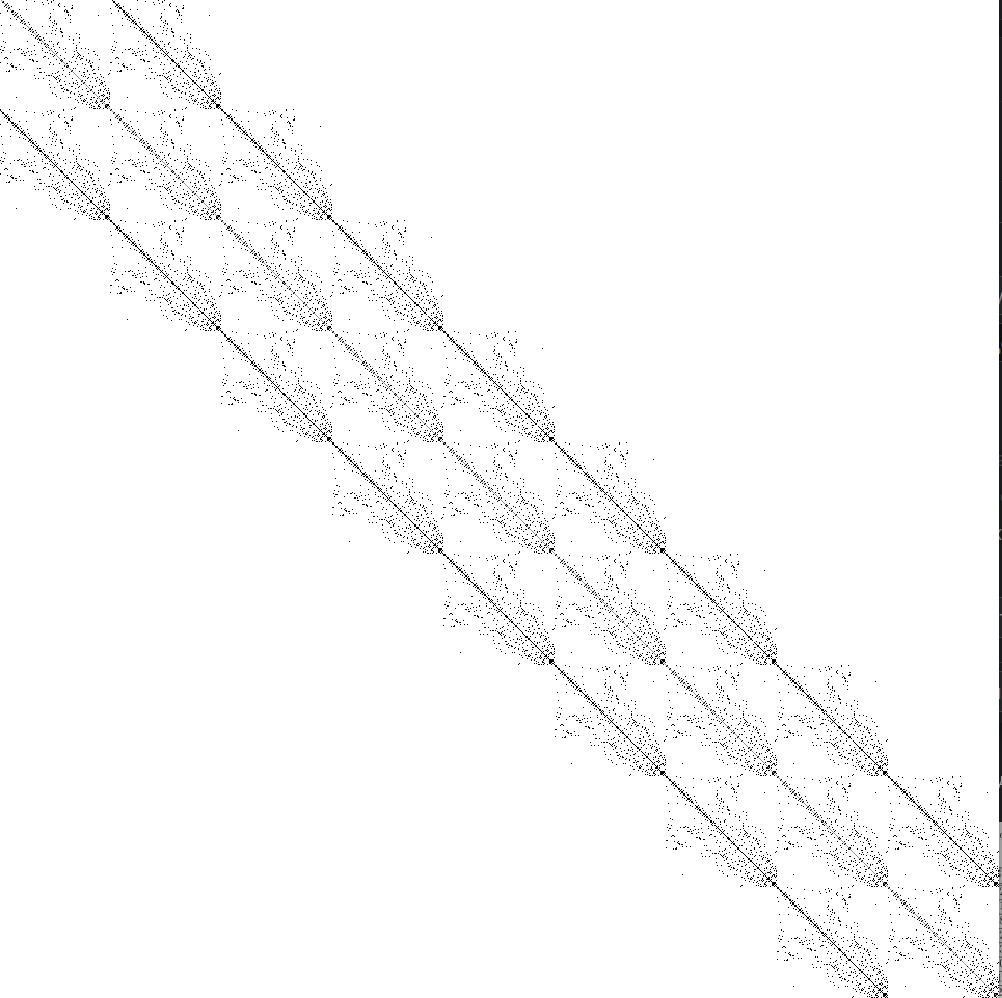
\includegraphics[scale=0.5]{A_g2_1_portait.png}
		\caption{Портрет матрицы A_g2_1.mtx}
	\end{figure}
	
\end{document}